\documentclass{article}
\usepackage[utf8]{inputenc}

\title{Interrupciones}
\author{Chrsitian Gallego Chaverra}
\date{June 2020}

\usepackage{natbib}
\usepackage{graphicx}

\begin{document}

\maketitle

\section{Que es una Interrupción}
Una interrupción es una señal recibida por el procesador de un ordenador, indicando que debe interrumpir el curso de ejecución actual y pasar a ejecutar un bloque de código especifico para tratar alguna situación.\cite{def}
Las interrupciones surgen de la necesidad que tienen los periféricos de enviar información al procesador. La primera técnica que se empleo fue que el propio procesador sondeara el dispositivo cada cierto tiempo para ver si había alguna comunicación pendiente para él. Esta técnica no fue del todo eficiente porque el procesador necesitaba un estimado de tiempo para el sondeo. Solucionaron este problema implementando el mecanismo de interrupciones; ya que en este caso el microprocesador no sondea ningún dispositivo sino que espera que le avisen (por medio de una interrupción) cuando existan comunicaciones para él por medio del IRQ. Las IRQ (Interrupt ReQuest) son líneas que llegan al controlador de interrupciones; un componente de hardware dedicado a la gestión de las interrupciones, y que puede estar integrado en el procesador principal o ser un circuito separado conectado al mismo. Este controlador de interrupciones debe ser capaz de habilitar o inhibir lineas de interrupción y establecer prioridades entre las distintas interrupciones habilitadas. 

\section{Tipos de Interrupciones}
Existen tres tipos de interrupciones:
\subsection{Interrupciones de hardware}
Estas interrupciones pueden ser internas o externas.
Las interrupciones internas son generadas por ciertos eventos que surgen durante la ejecución de un programa.
Este tipo de interrupciones son manejadas en su totalidad por el hardware y no es posible modificarlas.
Un ejemplo claro de este tipo de interrupciones es la que actualiza el contador del reloj interno de la computadora, el hardware hace el llamado a esta interrupción varias veces durante un segundo para mantener la hora actualizada.
Las interrupciones externas las generan los dispositivos periféricos, como pueden ser: teclado, impresoras, tarjetas de comunicaciones, etc. También son generadas por los coprocesadores.
No es posible desactivar a las interrupciones externas.
Estas interrupciones no son enviadas directamente a la CPU, sino que se mandan a un circuito integrado cuya función es exclusivamente manejar este tipo de interrupciones. El circuito, llamado PIC 8259A\cite{8259}, si es controlado por la CPU utilizando para tal control una serie de vías de comunicación llamadas puertos.

\begin{figure}[h]
\centering
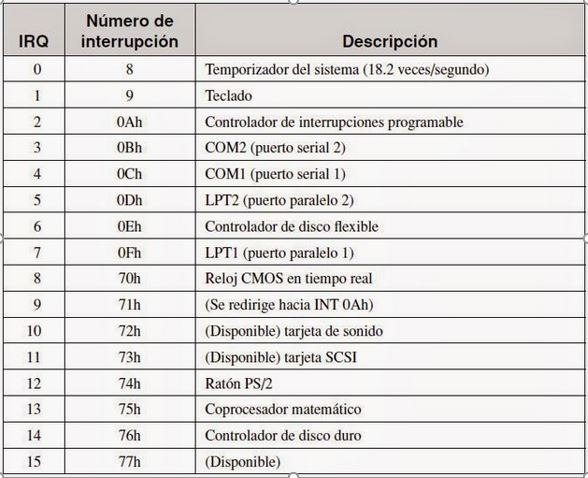
\includegraphics[scale=0.7]{interrupciones}
\caption{Interrupciones de hardware \cite{interHS}}
\label{fig:interrupciones}
\end{figure}

\subsection{Interrupciones de software}
Las interrupciones de software pueden ser activadas directamente por el ensamblador invocando al número de interrupción deseada con la instrucción INT\cite{int}.
El uso de las interrupciones nos ayuda en la creación de programas, utilizándolas nuestros programas son más cortos, es más fácil entenderlos y usualmente tienen un mejor desempeño debido en gran parte a su menor tamaño.
Este tipo de interrupciones podemos separarlas en dos categorías: las interrupciones del sistema operativo DOS y las interrupciones del BIOS.
La diferencia entre ambas es que las interrupciones del sistema operativo son más fáciles de usar, pero también son más lentas ya que estas interrupciones hacen uso del BIOS para lograr su cometido, en cambio las interrupciones del BIOS son mucho más rápidas, pero tienen la desventaja que, como son parte del hardware son muy específicas y pueden variar dependiendo incluso de la marca del fabricante del circuito.
La elección del tipo de interrupción a utilizar dependerá únicamente de las características que le quiera dar a su programa: velocidad (utilizando las del BIOS) o portabilidad (utilizando las del DOS).

\begin{figure}[h]
\centering
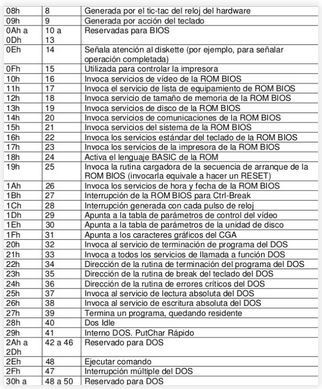
\includegraphics[scale=1.2]{interrupciones2}
\caption{Interrupciones de software \cite{interHS}}
\label{fig:interrupciones2}
\end{figure}

\subsection{Excepciones}
Las excepciones son un tipo de interrupción sincrónica típicamente causada por una condición de error en un programa, como por ejemplo una división entre 0 o un acceso inválido a memoria en un proceso de usuario. Normalmente genera un cambio de contexto a modo supervisor para que el sistema operativo atienda el error. Así pues, las excepciones son un mecanismo de protección que permite garantizar la integridad de los datos almacenados tanto en el espacio de usuario como en el espacio kernel. Cuando el Sistema Operativo detecta una excepción intenta solucionarla, pero en caso de no poder simplemente notificará la condición de error a la aplicación/usuario y abortará la misma. 

\section{Interrupción con Arduino}
El siguiente código empleamos el pin digital 10 para emular una onda cuadrada de intervalo 2s (1s ON y 1s OFF).
En cada interrupción actualizamos el valor de un contador. Posteriormente, en el bucle principal, comprobamos el valor del contador, y si ha sido modificado mostramos el nuevo valor.
Al ejecutar el código, veremos que en el monitor serie se imprimen números consecutivos a intervalos de dos segundos.

Para probar la interrupción en Arduino conectamos el pin 10 al 2 asociado a la interrupción 0, en la placa de Arduino, como se muestra en la figura 3.

\begin{figure}[h]
\centering
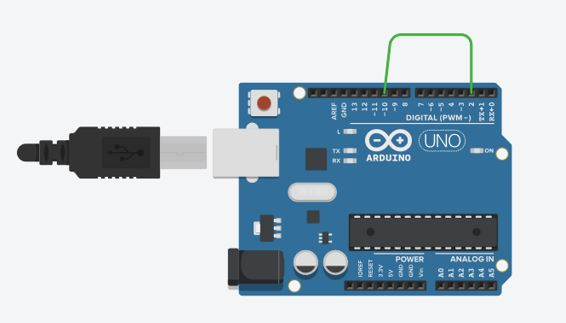
\includegraphics[scale=0.5]{interrupcionA}
\caption{Configuración de Arduino para la Interrupción}
\label{fig:interrupcionA}
\end{figure}

Luego en el código definimos los pines a utilizar y los contadores
El código y su ejecución están en el siguiente link de Tinkercad, donde se simulo la interrupción:

https://www.tinkercad.com/things/37e7SP8rarC-grand-rottis/editel 

\bibliographystyle{plain}
\bibliography{references}
\end{document}
